\documentclass[border=10pt]{standalone}
\usepackage[T1]{fontenc}
\usepackage[default]{sourcesanspro}
\usepackage{tikz}
\usepackage{xcolor}
\usetikzlibrary{positioning}

\begin{document}
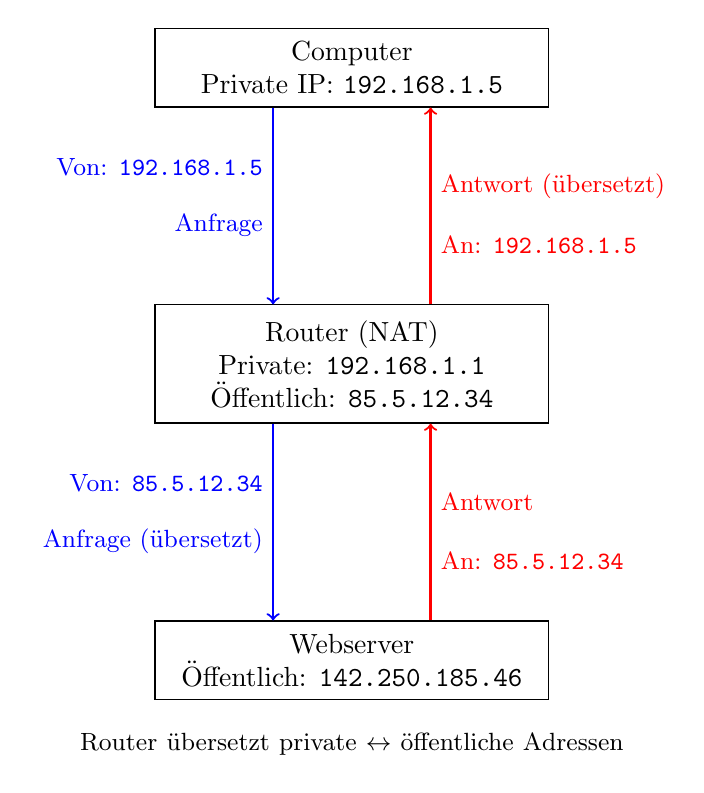
\begin{tikzpicture}[node distance=1.5cm, auto]
		% Nodes
		\node[draw, rectangle, minimum width=5cm, minimum height=1cm, align=center] (pc) {Computer\\Private IP: \texttt{192.168.1.5}};
		\node[draw, rectangle, minimum width=5cm, minimum height=1.5cm, below=2.5cm of pc, align=center] (router) {Router (NAT)\\Private: \texttt{192.168.1.1}\\\"Offentlich: \texttt{85.5.12.34}};
		\node[draw, rectangle, minimum width=5cm, minimum height=1cm, below=2.5cm of router, align=center] (server) {Webserver\\\"Offentlich: \texttt{142.250.185.46}};

		% Request arrows (blue, left side with labels on left)
		\draw[->, thick, blue] ([xshift=-1cm]pc.south) -- node[left, pos=0.6] {\small Anfrage} node[left, pos=0.3] {\small Von: \texttt{192.168.1.5}} ([xshift=-1cm]router.north);
		\draw[->, thick, blue] ([xshift=-1cm]router.south) -- node[left, pos=0.6] {\small Anfrage (\"ubersetzt)} node[left, pos=0.3] {\small Von: \texttt{85.5.12.34}} ([xshift=-1cm]server.north);

		% Response arrows (red, right side with labels on right)
		\draw[->, thick, red] ([xshift=1cm]server.north) -- node[right, pos=0.6] {\small Antwort} node[right, pos=0.3] {\small An: \texttt{85.5.12.34}} ([xshift=1cm]router.south);
		\draw[->, thick, red] ([xshift=1cm]router.north) -- node[right, pos=0.6] {\small Antwort (\"ubersetzt)} node[right, pos=0.3] {\small An: \texttt{192.168.1.5}} ([xshift=1cm]pc.south);

		\node[below=0.3cm of server, text width=8cm, align=center] {\small Router \"ubersetzt private $\leftrightarrow$ \"offentliche Adressen};
	\end{tikzpicture}
\end{document}
